\chapter{Teoria de conjuntos}

%Texto baseado em Topologia-Elon e \cite{munkres}.

Chamamos de \textbf{conjunto} uma coleção de objetos que satifazem uma propriedade comum. Usaremos letras maiúsculas $A, B, \ldots$ para representar  conjuntos, e letras minúsculas $a, b, \ldots$ para representar seus elementos.

A notação $x \in A$ (lê-se "$x$ pertence à $A$) significa que $x$ é um elemento de $A$. A notação $x \notin A$ (lê-se "$x$ não pertence à $A$) significa que $x$ não é um elemento de $A$.

Dados os elementos $a, e, i, o, u$ indica-se com $\{a, e, i, o, u\}$ o conjunto que é formado por estes elementos. Assim, por exemplo, $V= \{a, e, i, o, u\}$ é o conjunto das vogais do alfabeto português, quando representamos um conjunto desta forma dizemos que estamos representando o conjunto por enumeração de seus elementos.

Assim se denotarmos por $U$ o conjunto formado pelas letras do alfabeto português, como toda vogal é uma letra do alfabeto português, podemos representar o conjunto $V$ da seguinte forma:
\[V= \{x \in U | x \text{ é uma vogal}\}\]
aqui $x$ representa um elemento qualquer do conjunto $U$.

Esta segunda forma que usamos para descrever o conjunto $V$ é uma forma usual de descrever conjuntos na matemática, perceba que nela começamos pensando em um conjunto "grande" $U$ (que chamamos de conjunto universo) e em uma propriedade $P$ bem particular que alguns elementos deste conjunto satifaziam, e assim obtemos o conjunto $V$.

Além de relacionar elementos com conjuntos podemos relacionar dois conjuntos, uma forma de relacionar dois conjuntos é através da relação de \textit{inclusão}, que é descrita da seguinte forma, dados dois conjuntos $M$ e $N$, diremos que $M$ está contido em $N$ se todo elemento de $M$ é também um elemento de $N$, neste caso escrevemos $M \subset N$. 

Note que em nosso exemplo anterior $V \subset U$, já que toda vogal é também uma letra do alfabeto português. Outro exemplo: como $a$ é um elemento de $V$. Dizer que $a \in V$ é equivalente a afirmar que $\{a\} \subset V$.

\vskip0.4cm

Considerando três conjuntos quaisquer $A$, $B$ e $C$, a relação de inclusão entre eles possui das seguintes propriedades:

\textit{Reflexividade:} para todo conjunto A, tem-se que $A \subset A$.

\textit{Anti-simetria:} se $A \subset B$ e $B \subset A$ então, $A= B$.

\textit{Transitividade:} se $A \subset B$ e $B \subset C$ então, $A \subset C$.

\newpage

Notações:
\begin{itemize}
 \item Elemento $a$ pertence ao conjunto $A$: $\destaque{a \in A}$.
 \item Elemento $a$ não pertence ao conjunto $A$: $\destaque{a \notin A}$.
 \item Conjunto $A$ está contido no conjunto $B$: $\destaque{A \subset B}$.
 \item Conjunto $A$ contém o conjunto $B$: $\destaque{A \supset B}$.
 \item Conjunto $A$ é subconjunto próprio do conjunto $B$: $\destaque{A \varsubsetneq B}$.
 \item O conjunto que não contém nenhum elemento será denotado por $\destaque{\emptyset}= \{ \}$ = conjunto vazio.
\end{itemize}

\vskip0.4cm

 \begin{exem}
  Sejam $A= \{1, 2, 3, 4, 5 \}$ e $B=\{ 2, 3, 4\}$. Então $1 \in A$, mas $1 \notin B$. Além disso, temos que $B \subset A \Rightarrow A \supset B$.
 \end{exem}
 
 Os conjuntos são também representados através do diagrama de Veen-Euler, no qual basicamente desenhamos um retângulo para representar o conjunto universo, dentro deste retângulo desenhamos um círculo para representar o conjunto, e dentro do círculo escrevemos os elementos que pertencem a este conjunto.
 
 \begin{exem}
 Consideremos o conjunto das vogais como sendo nosso conjunto universo, assim dentro dele podemos considerar os conjuntos $A= \{a,e, i\}$, e $B=\{a, o, u\}$  estes conjuntos serão representados através do diagrama de Veen-Euler da seguinte forma:
 
 \begin{center}
  \begin{venndiagram2sets}[labelOnlyA={e i},labelOnlyB={o u},labelAB={a}]
  \end{venndiagram2sets}
  \end{center}

 
 \end{exem}

 \vskip0.4cm
 
\section{Operações entre conjuntos}

Dados $A$ e $B$ conjuntos arbitrários dentro do conjunto universo $U$, definimos as seguintes operações entre estes conjuntos:
\begin{itemize}
 \item União: 
 $A \cup B=\{x / x \in A \text{ ou } x \in B\}.$
 
 \begin{venndiagram2sets}
  \fillA \fillB
 \end{venndiagram2sets}

 \vskip0.4cm
 \newpage
 
 \item Interseção: 
 $A \cap B=\{x / x \in A \text{ e } x \in B\}.$
 
 \begin{venndiagram2sets}
  \fillACapB
 \end{venndiagram2sets}
 
 \vskip0.4cm
 
 \item Diferença:
 
 $A - B= \{x | x \in A \text{ e } x \notin B\}.$
 
 \begin{venndiagram2sets}
  \fillANotB
 \end{venndiagram2sets}
 
 $B - A= \{x | x \notin A \text{ e } x \in B\}.$
 
 \begin{venndiagram2sets}
  \fillBNotA
 \end{venndiagram2sets}
 
 \vskip0.4cm
 
 \item Complementares:
 
 $\overline{A}= A^{C}= \{x \in U / x \notin A\}$
 
 \begin{venndiagram2sets}
  \fillNotA
 \end{venndiagram2sets}
 
 $\overline{B}= B^{C}= \{x \in U / x \notin B\}$
 
 \begin{venndiagram2sets}
  \fillNotB
 \end{venndiagram2sets}
 
 $\overline{A \cap B}= (A\cap B)^{C}= \{x \in U / x \notin (A\cap B)\}$
 
 \begin{venndiagram2sets}
  \fillNotAorNotB
 \end{venndiagram2sets}
 
 $\overline{A\cup B}= (A\cup B)^{C}= \{x \in U / x \notin (A\cup B)\}$
 
 \begin{venndiagram2sets}
  \fillNotAorB
 \end{venndiagram2sets}
 
 \vskip0.4cm
 
 \item Produto cartesiano:
 $A \times B= \{(a, b)| a \in A \text{ e } b \in B \}$
 
 O produto cartesiano de dois conjuntos pode ser representado usando eixos coordenados, como mostra o exemplo abaixo. Esta representação é particularmente útil para representar os gráficos de funções de $\R$ para $\R$.
 
 \begin{exem}
  Dados os conjuntos $A= \{1, 2, 3, 4, 5 \}$ e $B=\{ 2, 3, 4, 6\}$, podemos representá-los através do seguinte diagrama de Venn-Euler:
  \begin{center}
  \begin{venndiagram2sets}[labelOnlyA={1 5},labelOnlyB={6},labelAB={2  3  4}]
  \end{venndiagram2sets}
  \end{center}
  
  Considerando os conjuntos $A$ e $B$ dados, ao aplicar as operações de conjuntos entre eles obtemos os seguintes conjuntos, e suas respectivas representações através do diagrama de Venn-Euler:
  
  \vskip0.4cm
  
  $A \cup B=\{ 1, 2, 3, 4, 5 \}$
  
  \begin{venndiagram2sets}[labelOnlyA={1 5},labelOnlyB={6},labelAB={2  3  4}]
  \fillA \fillB
  \end{venndiagram2sets}
  
  \vskip0.4cm
  
  $A \cap B=\{2, 3, 4 \}$
  
  \begin{venndiagram2sets}[labelOnlyA={1 5},labelOnlyB={6},labelAB={2  3  4}]
  \fillACapB
  \end{venndiagram2sets}
  
  \vskip0.4cm
  
  $A - B= \{1, 5 \}$
  
  \begin{venndiagram2sets}[labelOnlyA={1 5},labelOnlyB={6},labelAB={2  3  4}]
  \fillANotB
  \end{venndiagram2sets}
  
  \vskip0.4cm
  
  \begin{eqnarray*}
   A \times B= \{(1, 2), (1, 3), (1, 4), (1, 6), (2, 2), (2, 3), (2, 4), (2, 6), (3, 2), (3, 3), (3, 4), (3, 6), \\
    (4, 2), (4, 3), (4, 4), (4, 6), (5, 2), (5, 3), (5, 4), (5, 6) \}
  \end{eqnarray*}
  
  \begin{figure}[H]
 \centering
    \fbox{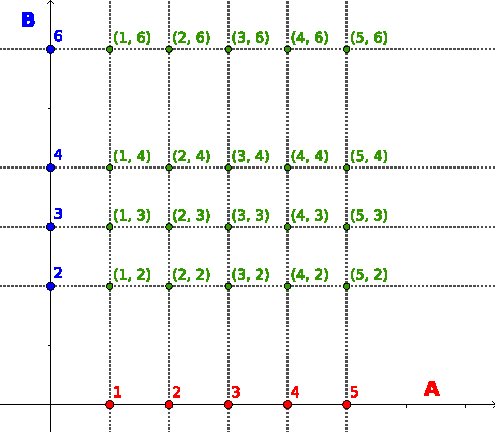
\includegraphics[width=7cm]{../Topicos/Figuras/ProdCartConj.pdf}}
    \caption{Produto cartesiano dos conjuntos $A$ e $B$}
  \end{figure}
  
 \end{exem}
 
 \vskip0.4cm
 
 A \textbf{cardinalidade} de um conjunto $A$ qualquer, é o número de elementos deste conjunto. Denotada por: $n(A)$, $|A|$ ou $\# A$. 
 
 Note que: $n(\emptyset)= \# \emptyset= 0$.
 
 Dados dois conjuntos $A$ e $B$ quaisquer é importante observar que:
 \vskip0.3cm
 \colorbox{azul}{
 \begin{minipage}{14.5cm}
 \begin{center}
 A cardinalidade da união destes dois conjuntos é dada por:
  \[\#(A \cup B)= \# A + \# B - \#(A \cap B) \ .\]
 \end{center}
 \end{minipage}}
 \vskip0.3cm
 
 Esta fórmula irá nos ajudar a resolver muitos problemas de teoria de conjuntos.
 
 \newpage
 
 Dada uma família $\mathcal{A}$ de conjuntos, ou seja, dado um conjunto $\mathcal{A}$ de conjuntos, temos:
 \item União de todos os conjuntos que são elementos de $\mathcal{A}$:
 $$\bigcup_{A \in \mathcal{A}} A = \{x| x \in A \text{ para algum } A \in \mathcal{A}\}$$
 \item Interseção de todos os conjuntos que são elementos de $\mathcal{A}$:
 $$\bigcap_{A \in \mathcal{A}} A = \{x| x \in A \text{ para todo } A \in \mathcal{A}\}$$
\end{itemize}

\begin{prop}
Sejam $A$, $B$ e $C$ conjunto arbitrários, temos que:
\begin{itemize}
 \item $\emptyset \subset A$, $\forall A$
 \item $A \cup \emptyset= A$ e $A \cap \emptyset= \emptyset$
 \item $A \cap (B \cup C) = (A \cap B) \cup (A \cap C)$
 \item $A \cup (B \cap C) = (A \cup C) \cap (A \cup C)$
 \item $A - (B \cup C) = (A - B) \cap (A - C)$ (lei de DeMorgan)
 \item $A - (B \cap C) = (A - B) \cup (A - C)$ (lei de DeMorgan)
 \item $\bigcap_{\alpha \in J}(U_{\alpha} \cap Y) = (\bigcap_{\alpha \in J} U_{\alpha}) \cap Y$
 
  $$(U_1 \cap Y) \cap \cdots \cap (U_n \cap Y) = (U_1 \cap \cdots \cap U_n) \cap Y$$
  
 \item $\bigcup_{\alpha \in J}(U_{\alpha} \cap Y) = (\bigcup_{\alpha \in J} U_{\alpha}) \cap Y$
 
 $$(U_1 \cap Y) \cup \cdots \cup (U_n \cap Y) = (U_1 \cup \cdots \cup U_n) \cap Y$$
 
 \item $(U \times V) \cap (A \times B) = (U \cap A) \times (V \cap B)$
 
 \item $X - \bigcap_{\alpha \in J} A_{\alpha} = \bigcup_{\alpha \in J}(X - A_{\alpha})$
 
 \item $X - \bigcup_{i= 1}^{n} A_i = \bigcap_{i = 1}^{n}(X - A_i)$
 
\end{itemize}
\end{prop}

 


 

% \begin{enumerate}[a)]
%  \item 
%  \end{enumerate}
 




